\documentclass[review]{vgtc}

\graphicspath{{figures/}{pictures/}{images/}{./}}

% Keep the official VGTC template metrics and typography.
\usepackage{times}
\renewcommand*\ttdefault{txtt}
\usepackage{mathptmx}

\usepackage{amsmath}
\usepackage{amssymb}
\usepackage{enumitem}
\hyphenation{Static-Lock Ego-Anchor}
\usepackage{array}
\usepackage{booktabs}
\usepackage{multirow}
\usepackage{tabularx}
\usepackage{xcolor}
\usepackage{placeins}

\onlineid{1118}
\vgtccategory{System}
\vgtcinsertpkg

\title{EgoAnchor: Zero-Shot Dynamic Anchoring of Everyday Objects in Passthrough Mixed Reality}

\author{%
  Hailin Ji 
  \thanks{e-mail: \texttt{jihailin@mail.bnu.edu.cn}} \\
  School of Artificial Intelligence \\
  Beijing Normal University \\
  Beijing, China
  \and Yifeng Chen 
  \thanks{e-mail: \texttt{yfchen@mail.bnu.edu.cn}} \\
  School of Artificial Intelligence \\
  Beijing Normal University \\
  Beijing, China
  \and Haonian Wang
  \thanks{e-mail: \texttt{haonianwang@mail.bnu.edu.cn}} \\
  School of Artificial Intelligence \\
  Beijing Normal University \\
  Beijing, China
  \and Yiran Zhang 
  \thanks{e-mail: \texttt{zhangyiran@mail.bnu.edu.cn}} \\
  School of Artificial Intelligence \\
  Beijing Normal University \\
  Beijing, China
  \and Hongwen Zhang 
  \thanks{Corresponding author; e-mail: \texttt{zhanghongwen@bnu.edu.cn}} \\
  School of Artificial Intelligence \\
  Beijing Normal University \\
  Beijing, China
  \and Yanhong Luo 
  \thanks{Corresponding author; e-mail: \texttt{273961431@xbmu.edu.cn}} \\
  College of Electrical Engineering \\
  Northwest Minzu University \\
  Lanzhou, China
}

\abstract{%
Zero-shot six-degree-of-freedom (6DoF) pose estimation can localize novel everyday objects, but its asynchronous, low-rate, and variable-quality outputs cannot directly provide continuous, stable anchors in passthrough mixed reality (PMR). We present EgoAnchor, an egocentric system for zero-shot dynamic object anchoring. Its perception backend produces camera-frame observations with visual consistency scores, while the runtime transforms them into capture-time world-frame states and maintains reliable anchors for rendering and occlusion recovery. We implement EgoAnchor on Meta Quest 3 and evaluate it through controlled benchmarks against a hardware-tracked reference, component ablations, and a within-subject study with 24 participants. Compared with the baselines, EgoAnchor yields lower static registration and occlusion recovery errors and lower lag-aligned trajectory residuals, but higher motion onset latency. Participants also rate it higher for visual integration, interaction trust, and willingness to rely on the system. We will release the source code upon acceptance.
}

\keywords{passthrough mixed reality, dynamic object anchoring, 6DoF pose estimation, runtime systems, user perception}

% ===== Teaser =====
\teaser{%
  \centering
  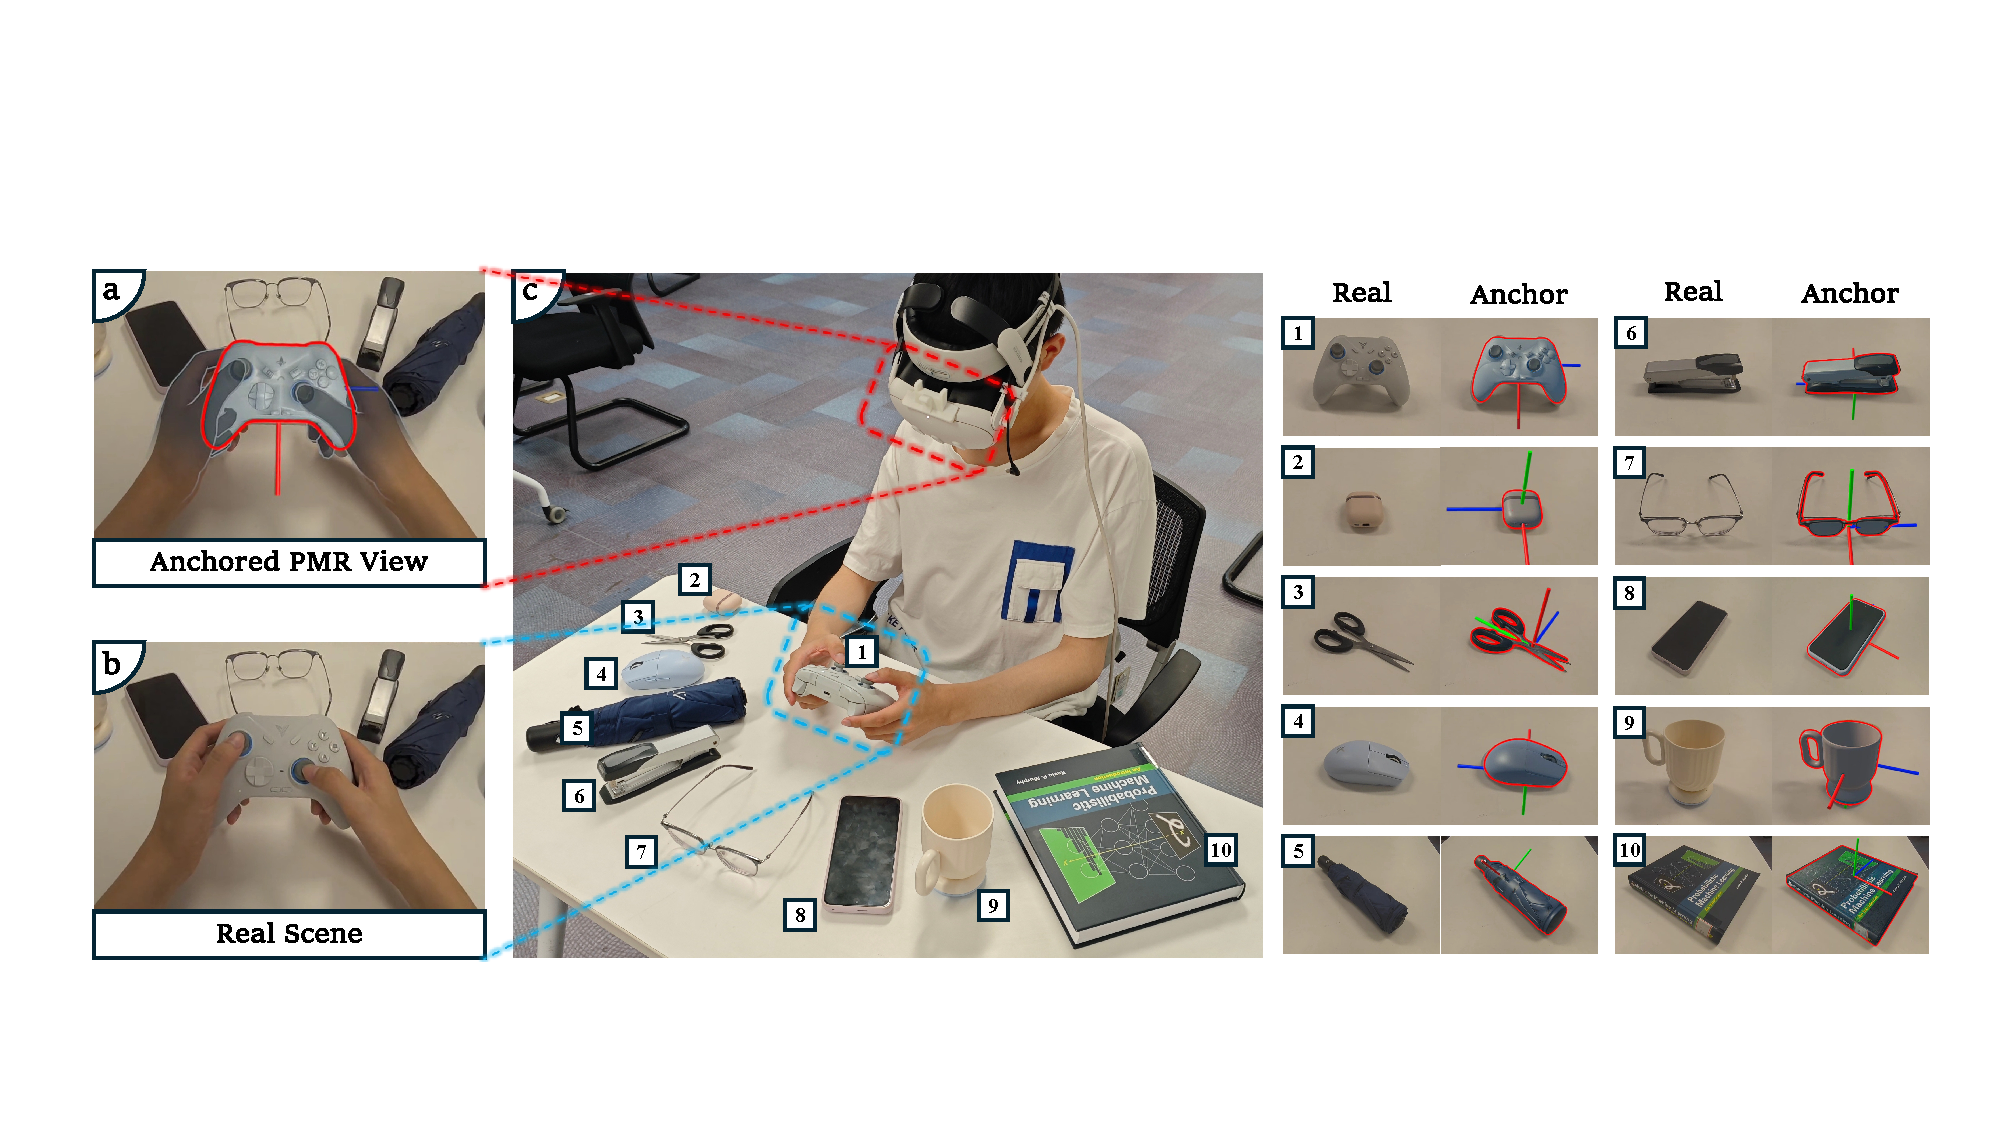
\includegraphics[width=\linewidth]{figures/teaser.pdf}
  \caption{Zero-shot dynamic anchoring of everyday objects with EgoAnchor. (a) Egocentric augmented views; (b) passthrough views at the same moments; (c) third-person interaction views. Labels 1--10 correspond to the objects on the right, each shown as the real object (Real) and its anchored visualization (Anchor). In (a) and the Anchor examples, red contours and local axes indicate the estimated 6DoF anchors. The objects are a game controller, earbud case, scissors, wireless mouse, umbrella, stapler, glasses, smartphone, mug, and book, spanning varied scales, geometries, and appearances.}
  \label{fig:teaser}
}

\begin{document}

\firstsection{Introduction}\label{sec:introduction}
\maketitle

Passthrough mixed reality (PMR) allows virtual content to be attached to physical entities around the user and supports applications such as procedural instructions, interaction guidance, state visualization, and near-object interaction. These applications require more than object category recognition. They must continuously maintain an object-level spatial reference frame as the object moves. When the user moves their head, manipulates the object by picking it up, rotating it, or translating it, or briefly occludes it, the virtual overlay should preserve a consistent six-degree-of-freedom (6DoF) spatial relationship with the physical object. Conventional spatial anchors are designed mainly for static environments and cannot represent object motion. Object-level dynamic anchoring with real-time updates is therefore a fundamental capability for object-centric MR applications~\cite{selfblending2026,gradualreality2024}.

Existing approaches provide partial support at different levels. Native object-tracking interfaces on commercial headsets offer tight platform integration, but their supported object categories, model specifications, and runtime behavior are constrained by platform-defined requirements, as in Apple Vision Pro and Meta Quest. Fiducial markers such as AprilTag and ArUco, as well as dedicated hardware trackers such as HTC Tracker, provide stable localization but require physical modification of the target or attachment of extra hardware. Recent advances in open-vocabulary detection, temporal segmentation, stereo matching, and model-based zero-shot 6DoF pose estimation enable visual localization of rigid objects with known 3D models~\cite{groundingdino2025,cutie2024,fastfoundationstereo2026,foundationpose2024,gigapose2024}. These foundation models broaden the scope of visual localization, but their outputs remain discrete and asynchronous camera-frame observations tied to specific image capture times. They cannot directly serve as stable object anchors for MR applications.

Using visual poses directly as object anchors introduces several runtime problems. First, an asynchronous result has already accumulated processing latency when it reaches the rendering client. If it is composed with the headset pose at arrival time, headset motion is incorrectly interpreted as object motion, producing head-motion coupling error. Second, even after temporal alignment, candidate poses can jump because of occlusion, depth noise, or geometric mismatch. Directly accepting such candidates causes rendering jitter. Finally, a low-rate, irregular, and noisy pose stream cannot directly support high-rate per-frame rendering. The runtime must also manage stationary and moving states, state transitions, brief observation failures, and reacquisition. A single-frame pose estimate is therefore insufficient to form a persistent object anchor.

We address these problems with EgoAnchor, an egocentric system for zero-shot dynamic object anchoring in PMR. The perception backend organizes open-vocabulary detection, temporal segmentation, stereo depth estimation, and zero-shot pose estimation into a continuous pipeline. It evaluates each observation using a visibility-gated color and depth (VCD) score. The anchoring runtime transforms asynchronous candidate poses into world-frame observations at their capture times and maintains reliable object states for real-time rendering. It continues to produce usable anchors while the object moves, remains stationary, or becomes briefly unobserved. EgoAnchor requires no physical marker or object-specific training. A new target needs only a 3D CAD model and a short text description, and the model can come from an existing digital asset or offline image-based reconstruction.

Our main contributions are:
\begin{enumerate}[leftmargin=1.8em,itemsep=1pt,topsep=2pt]
  \item \textbf{EgoAnchor system:} A system that converts asynchronous, low-rate zero-shot camera-frame observations into continuous world-frame dynamic anchors.
  \item \textbf{Anchoring perception and runtime:} A VCD measure for per-observation reliability, combined with capture-time alignment, time-indexed state estimation, and stationary locking to maintain continuous and recoverable runtime output.
  \item \textbf{System evaluation:} Controlled benchmarks against a hardware-tracked reference, ablations of key components, and a within-subject study with 24 participants that quantify system performance, design tradeoffs, and user perception.
\end{enumerate}

\section{Related Work}\label{sec:related-work}

\subsection{Object Anchoring in MR}

Object anchoring establishes an object-level spatial reference for a physical entity so that virtual content remains attached as the object moves. Early methods mainly estimate object poses from fiducial markers such as AprilTag and ArUco~\cite{apriltag2011,aruco2014}. However, they require physical modification of the target and are difficult to apply to diverse everyday objects in open environments.

Consumer MR platforms now provide markerless object recognition and tracking. Azure Object Anchors\footnote{\href{https://learn.microsoft.com/en-us/dynamics365/mixed-reality/guides/pc-app-anchor-object}{Azure Object Anchors}}, Vuforia Model Targets\footnote{\href{https://developer.vuforia.com/library/vuforia-engine/images-and-objects/model-targets/model-targets/}{Vuforia Model Targets}}, Apple Vision Pro\footnote{\href{https://developer.apple.com/documentation/visionos/implementing-object-tracking-in-your-app}{Apple object tracking}}, and Meta Quest\footnote{\href{https://developers.meta.com/horizon/documentation/native/android/mobile-dynamic-object-tracker/}{Meta dynamic object tracking}} use onboard sensing and target models to establish object-level spatial states. These systems commonly require proprietary scans or offline target configuration and remain limited by supported object types and platform interfaces. Academic work further combines headset tracking, spatial mapping, cameras, and depth sensing to localize scene assets, register known objects, and track objects continuously~\cite{fan2021assettracking,doughty2022hmdegopose,pollabauer2023hololens,martingomez2024sttar,trojak2025mixedpose,greene2025markerless,trojak2026markerless,gbot2024}. These studies demonstrate the feasibility of object-level tracking with headset sensing, but they often depend on specific objects, task priors, dedicated hardware, or platform configuration. They therefore provide limited support for flexibly adding diverse everyday objects in open environments~\cite{hurt2025surrealitycv}.

\subsection{6DoF Object Pose Estimation and Tracking}

6DoF object pose estimation recovers the pose of a rigid object relative to the camera from visual observations and provides the perceptual basis for dynamic object anchoring~\cite{aguirrezabal2026survey}. Research has progressed from traditional methods based on local geometric feature matching to known-instance estimators that use RGB-D fusion, dense geometric regression, symmetry modeling, and self-supervised learning~\cite{densefusion2019,epos2020,gdrnet2021,self6d2020}. Recent methods further extend pose estimation to novel objects and zero-shot settings~\cite{gen6d2022,megapose2022,lin2024sam6d,ornek2024foundpose,moon2025coop,foundationpose2024}. Particle filters and multi-frame geometric constraints can also maintain temporal object states across frames~\cite{poserbpf2021,bundletrack2021}.

Visual foundation models further extend object perception in open environments. Open-vocabulary detection enables semantic target specification through natural language~\cite{owlvit2022,glip2022,groundingdino2025,yoloe2025}; video object segmentation maintains object identity and contours across frames~\cite{xmem2022,cutie2024}; and modern stereo matching improves depth recovery and cross-domain generalization in complex scenes~\cite{raftstereo2021,igevstereo2023,fastfoundationstereo2026}. Together, these capabilities make zero-shot visual localization of everyday object instances increasingly practical. However, they mainly address local perception and optimization in the camera frame. In MR, visual observations must be transformed into stable and continuous world-frame object states before they can serve as persistent object anchors.

\subsection{Temporal Alignment in XR}

Image capture, algorithmic inference, and network transmission introduce processing latency in XR systems. The latest state available for rendering can therefore correspond to an observation earlier than the current display time, and end-to-end latency can vary with system load and computation~\cite{diluca2010latency,mrloop2022,stauffert2020mtp}. A common strategy for resolving the mismatch between state timestamps and display time is \emph{predictive tracking}. It predicts or extrapolates an available state to the current or expected display time using a motion model, reducing dynamic registration error caused by processing and display latency~\cite{azuma1994improving,laviola2003double,pvt2023,yoon2022headmotion}.

Another strategy retains timestamped state records and queries or interpolates them at a specified historical time. Prior AR systems use timestamp synchronization, sampling-time adjustment, interpolation, or extrapolation to temporally register data streams with different latencies~\cite{jacobs1997latency}. OpenXR's \texttt{xrLocateSpace} interface\footnote{\href{https://registry.khronos.org/OpenXR/specs/1.1/man/html/xrLocateSpace.html}{OpenXR xrLocateSpace}} also distinguishes future prediction from a \emph{historical state query}. For a future time, the runtime returns its latest predicted spatial state. For a past time, it returns its current best estimate of the state at that historical time. Predictive tracking reduces state phase lag, whereas a historical state query recovers spatial geometry at a past time. The two approaches therefore make different temporal alignment tradeoffs.

\section{EgoAnchor System}\label{sec:system}

\subsection{System Overview}

EgoAnchor specifies a target using a short text description and an offline 3D model, without physical markers or object-specific training. The perception backend continuously generates camera-frame pose observations with reliability scores. The anchoring runtime transforms them into world-frame poses at their capture times and maintains object anchors at the rendering rate.

The runtime explicitly distinguishes image capture time $t_f$, candidate arrival time $t_a$, and rendering time $t_r$. Throughout the paper, $T_a^b\in\mathrm{SE}(3)$ denotes a rigid transformation from coordinate frame $a$ to frame $b$. The symbols $w$, $c$, and $o$ denote the world, left-camera, and local object frames, respectively. Filtered states and application-level outputs are denoted by $\widehat{T}$ and $\widetilde{T}$. Fig.~\ref{fig:arch} shows the system responsibilities and asynchronous data flow.

\begin{figure*}[t]
  \centering
  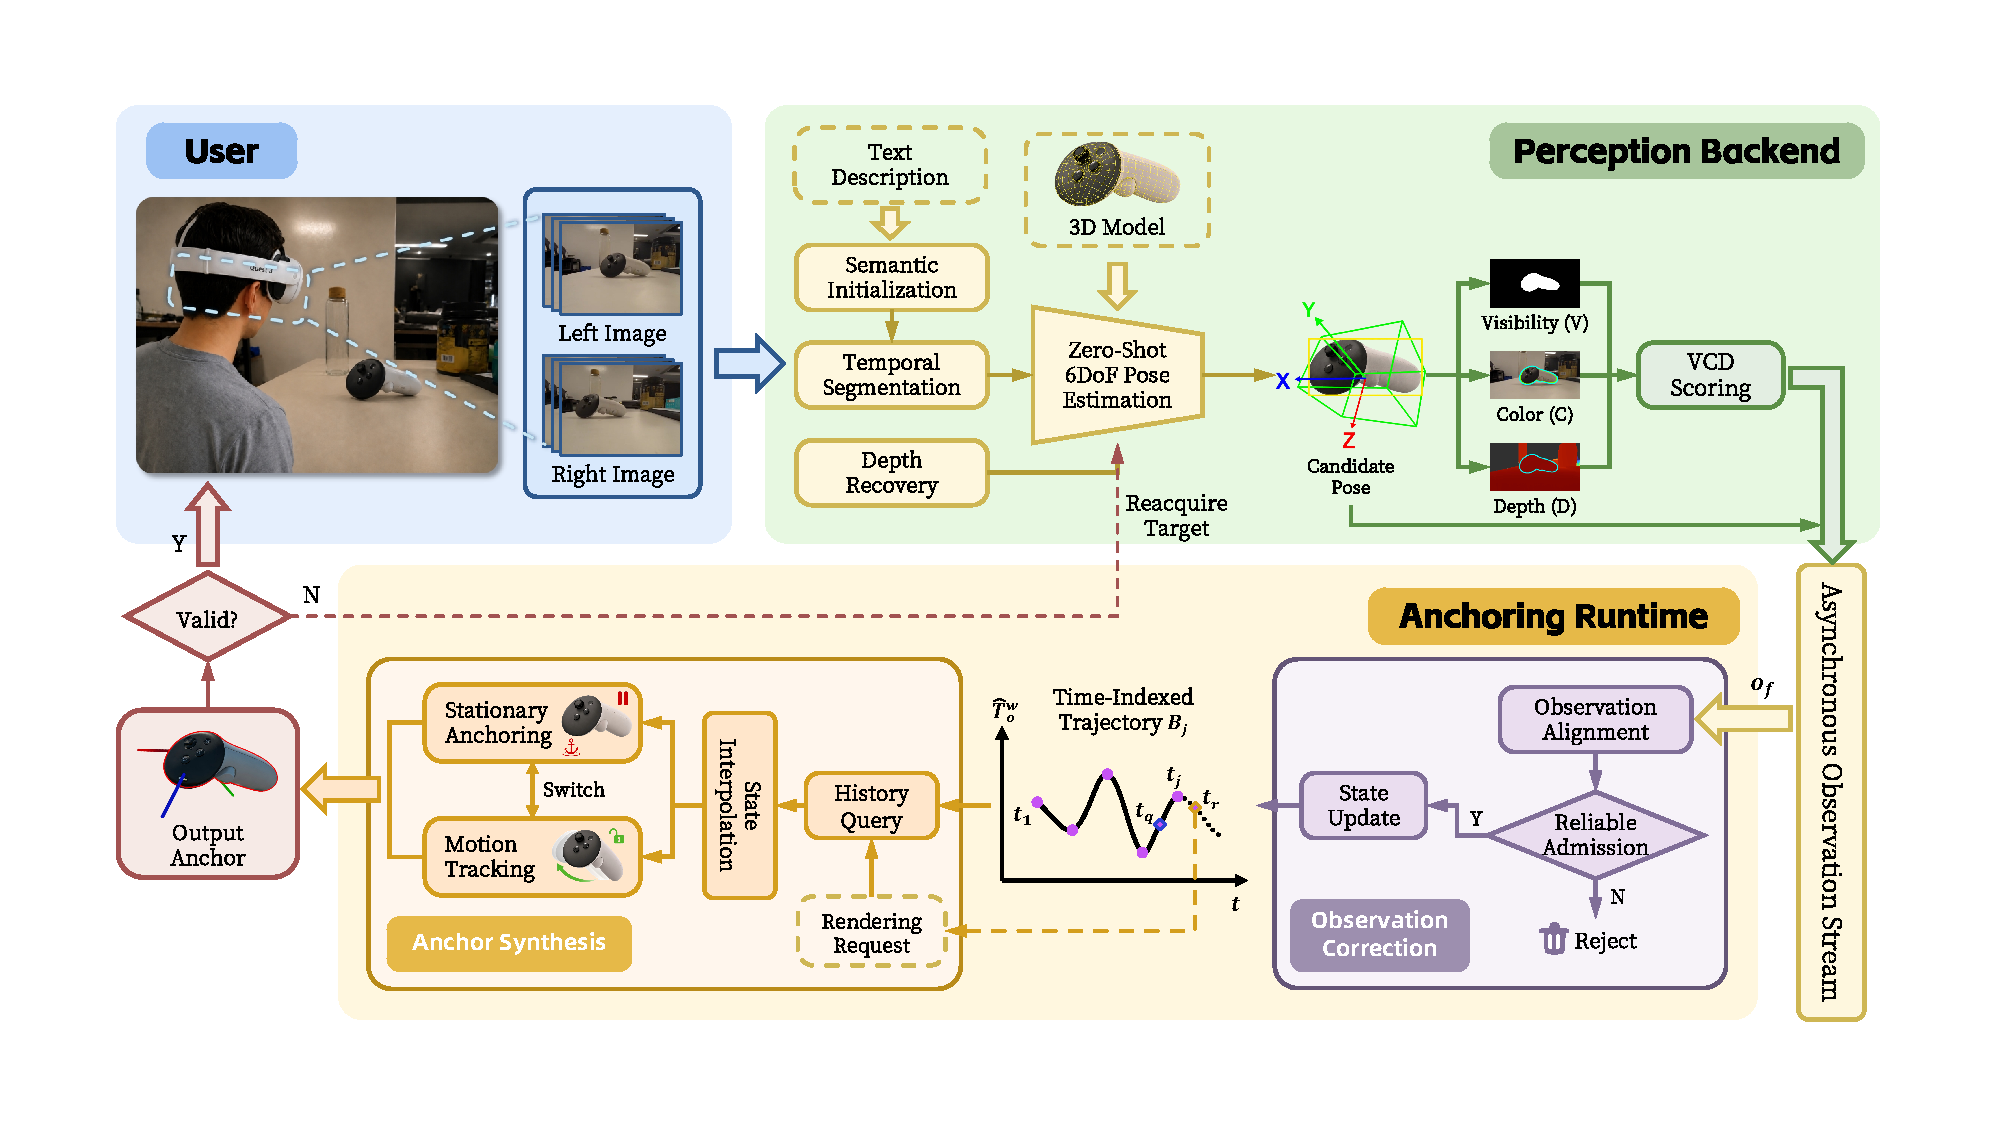
\includegraphics[width=\textwidth]{figures/pipeline_en.pdf}
  \caption{EgoAnchor architecture and asynchronous data flow. From stereo images, a text description, and a 3D model, the backend performs semantic initialization, temporal segmentation, stereo depth recovery, and zero-shot 6DoF pose estimation, then scores reliability from visibility (V), color (C), and depth (D). At the runtime, each asynchronous observation $o_f$ is transformed using the capture-time camera pose and admitted into a time-indexed trajectory $\mathcal{B}_j$. Each rendering frame interpolates the trajectory at historical query time $t_q$ and switches between dynamic tracking and stationary locking based on motion and observation support. Prolonged loss of reliable observations triggers reacquisition.}
  \label{fig:arch}
\end{figure*}

\subsection{Perception Backend}\label{sec:perception}

\textbf{Input and observation representation.}
Given headset stereo images $I_f = (I_f^L, I_f^R)$, a text description $Q_o$ of the target, and its 3D geometric model $G_o$, the perception backend forms an observation tuple for each processed frame:
\begin{equation}
o_f = (f, t_f, T_{o,f}^{c}, R_f),
\label{eq:observation}
\end{equation}
where $f$ is a monotonically increasing frame identifier assigned by the headset, $T_{o,f}^{c}$ is the 6DoF target pose in the left-camera frame, and $R_f \in [0,1]$ is the reliability score of the observation. The sequence $\{o_f\}$ forms the asynchronous observation stream between the two layers.

\subsubsection{Perception Pipeline for Anchoring}

The pipeline sequentially establishes the target identity, metric depth, and camera-frame pose.

\textbf{Semantic initialization.}
At the initialization frame $f_0$, an open-vocabulary detector~\cite{yoloe2025} obtains the target mask from the left image and text description:
\begin{equation}
M_{f_0} = \operatorname{Detect}(I_{f_0}^{L}, Q_o),
\label{eq:detect}
\end{equation}
Here, $f_0$ is the first frame with both a valid mask and sufficient depth coverage. The system selects a new $f_0$ when tracking fails and reacquisition is triggered.

\textbf{Temporal segmentation.}
The initial mask initializes a video object segmentation network~\cite{cutie2024}, which then propagates the target identity across frames:
\begin{equation}
(M_f, H_f) = \operatorname{Seg}(I_f^{L}, H_{f-1}), \qquad f > f_0,
\label{eq:seg}
\end{equation}
where $H_f$ is the temporal appearance memory that keeps pose estimation associated with the same target instance.

\textbf{Stereo depth estimation.}
A stereo matching network predicts disparity from the rectified stereo images and recovers metric depth:
\begin{equation}
d_f = \operatorname{Stereo}(I_f^{L}, I_f^{R}), \qquad Z_f = \frac{b f_x}{d_f},
\label{eq:depth}
\end{equation}
where $b$ is the stereo baseline and $f_x$ is the focal length in pixels.

\textbf{Zero-shot pose estimation.}
A model-based estimator~\cite{foundationpose2024} recovers the camera-frame pose from the mask, depth map, and 3D model:
\begin{equation}
T_{o,f}^{c} =
\begin{cases}
\operatorname{Reg}(M_f, Z_f, G_o), & \text{registration}, \\
\operatorname{Track}(M_f, Z_f, G_o, T_{o,f^-}^{c}), & \text{tracking},
\end{cases}
\label{eq:pose}
\end{equation}
Global registration runs only during initialization and reacquisition. For subsequent frames, the previous processed-frame result initializes local pose tracking.

\subsubsection{Per-Observation VCD Scoring}

Local occlusion and observation noise can cause zero-shot pose optimization to produce candidates that are inconsistent with the image evidence. VCD follows a render-and-compare paradigm~\cite{deepim2018,latentfusion2020,focalpose2022} and combines visibility (V), color (C), and depth (D) evidence to assess each candidate pose.

\textbf{Visibility gating.}
Let $M_f^{\mathrm{rnd}}$ denote the model mask rendered at the candidate pose. We define:
\begin{equation}
\Omega_f = M_f \cap M_f^{\mathrm{rnd}}, \quad \Omega_f^{\circ} = \operatorname{Erode}(\Omega_f), \quad V_f = \frac{|\Omega_f|}{|M_f^{\mathrm{rnd}}|},
\label{eq:visibility}
\end{equation}
Here, $V_f$ is the fraction of the rendered projection supported by the observed segmentation mask. The eroded core $\Omega_f^\circ$ reduces the influence of mixed pixels along object boundaries.

\textbf{Color and depth consistency.}
The color consistency score $S_f^C$ uses zero-mean normalized cross-correlation (ZNCC) in the CIE $L^*a^*b^*$ color space, with a lower weight on the luminance channel. Depth consistency combines a distance-adaptive absolute residual term $S_f^{D,\mathrm{abs}}$ with a surface-normal structure term $S_f^{D,\mathrm{str}}$ that is more robust to global depth bias:
\begin{equation}
S_f^D = (1-\alpha_f)\,S_f^{D,\mathrm{abs}} + \alpha_f\,S_f^{D,\mathrm{str}},
\label{eq:depth-score}
\end{equation}
where $\alpha_f$ is a fusion weight determined by local depth variation. For flat, weakly textured objects, the score relies mainly on absolute depth. Objects with pronounced geometric variation receive a stronger local structural constraint.

\textbf{Evidence aggregation.}
Let $K_f\subseteq\{C,D\}$ be the set of valid modalities in the current frame. The combined score is:
\begin{equation}
R_f = V_f \cdot
\begin{cases}
\exp\!\left(\dfrac{\sum_{k \in K_f} w_k \ln \max(S_f^{k}, \epsilon)}{\sum_{k \in K_f} w_k}\right), & K_f \neq \varnothing, \\[6pt]
1, & K_f = \varnothing.
\end{cases}
\label{eq:vcd}
\end{equation}
where $w_k$ is the modality weight and $\epsilon$ is a lower bound that prevents logarithmic singularities. Invalid modalities do not contribute to the aggregation. If neither color nor depth is available, the score reduces to $V_f$. Multiplicative visibility gating directly lowers candidate reliability under severe occlusion or projected geometric misalignment.

\subsection{Anchoring Runtime}\label{sec:anchoring}

The anchoring runtime converts the low-rate asynchronous candidate stream into object states synchronized with the display refresh. When a candidate arrives, the runtime transforms it into a world-frame pose at capture time and updates the trajectory. Each rendering frame synthesizes an anchor by interpolating this trajectory and manages stationary locking and validity according to motion cues and observation support. Candidate and rendering events are decoupled, so the output update rate is independent of the backend inference rate.

\subsubsection{Observation Correction}\label{sec:obs-update}

The runtime first transforms each candidate into a world-frame pose at capture time, then applies reliability and temporal admission before updating the state trajectory.

\textbf{Observation alignment.}
Candidate $T_{o,f}^{c}$ corresponds to image capture time $t_f$ but returns at $t_a$. If it is composed directly with the camera pose at arrival time, the intervening headset motion is incorrectly introduced into the object pose. Using frame identifier $f$, the runtime retrieves the cached capture-time camera pose $T_{c,f}^{w}$ and computes:
\begin{equation}
T_{o,f}^{w} = T_{c,f}^{w}
\begin{bmatrix}
1 & 0 & 0 & 0 \\
0 & -1 & 0 & 0 \\
0 & 0 & 1 & 0 \\
0 & 0 & 0 & 1
\end{bmatrix}
T_{o,f}^{c}
\begin{bmatrix}
-1 & 0 & 0 & 0 \\
0 & 1 & 0 & 0 \\
0 & 0 & 1 & 0 \\
0 & 0 & 0 & 1
\end{bmatrix},
\label{eq:capture-alignment}
\end{equation}
The two fixed matrices account for differences between computer-vision and graphics coordinate conventions and between their definitions of the local object axes.

\textbf{Reliability-based admission.}
Let $(t_j,T_{o,j}^{w},R_j)$ denote the $j$th admitted observation. The first candidate establishes a trajectory when it meets the reliability threshold. Each subsequent candidate must also have a later capture time:
\begin{equation}
R_f \geq R_{\min}, \qquad t_f > t_j \quad (j \geq 1).
\label{eq:admission}
\end{equation}
Candidates that fail these admission criteria do not update the internal state.

\textbf{State update.}
Each admitted observation triggers constant-velocity Kalman filter updates~\cite{kalman1960new} for translation and rotation, producing a smoothed state $\widehat{T}_{o,j}^{w}$ and the time-indexed trajectory:
\begin{equation}
\mathcal{B}_j = \{(t_i, \widehat{T}_{o,i}^{w})\}_{i=1}^{j}.
\label{eq:trajectory}
\end{equation}
The same update refreshes the motion statistics and reliability measures used by stationary locking.

\subsubsection{Anchor Synthesis}\label{sec:frame-output}

Trajectory $\mathcal{B}_j$ updates at a low and irregular rate, whereas the rendering pipeline requires an object state every frame at time $t_r$. The runtime first determines a historical query time $t_q$ adaptively, then reconstructs the object state by interpolating adjacent trajectory nodes.

\textbf{Historical state query.}
The age of the latest available node at rendering time $t_r$ is $\ell_r=t_r-t_j$. The runtime dynamically sets the query lag using an estimate $\bar{\ell}_r$ obtained through asymmetric exponential smoothing:
\begin{equation}
\ell_r = t_r - t_j, \qquad \Delta_r = \max(\Delta_{\min},\, s\,\bar{\ell}_r), \qquad t_q = t_r - \Delta_r.
\label{eq:target-time}
\end{equation}
Here, $\Delta_{\min}$ is the minimum query lag, $s$ is a scaling factor, and $t_q$ is the historical query time used for state reconstruction. This strategy increases the likelihood that $t_q$ lies between two available trajectory nodes.

\textbf{State interpolation.}
When $t_i\leq t_q\leq t_{i+1}$, the runtime geometrically interpolates the object pose between adjacent trajectory nodes:
\begin{equation}
\lambda_q = \frac{t_q - t_i}{t_{i+1} - t_i}, \qquad
\widehat{T}_o^w(t_q) = \operatorname{Interp}(\widehat{T}_{o,i}^{w}, \widehat{T}_{o,i+1}^{w}; \lambda_q),
\label{eq:history-interp}
\end{equation}
Translation uses linear interpolation (LERP), and rotation uses quaternion spherical linear interpolation (SLERP). If the query time falls outside the available trajectory interval, the runtime holds the nearest endpoint state.

\textbf{Output modes.}
To suppress small disturbances while the object is stationary, EgoAnchor switches adaptively between dynamic tracking and stationary locking:
\begin{equation}
\widetilde{T}_o^w(t_r) = \begin{cases}
\widehat{T}_o^w(t_q), & \text{tracking}, \\
T_{o,\mathrm{lock}}^w, & \text{locking}.
\end{cases}
\label{eq:staticlock}
\end{equation}

\subsubsection{Stationary Locking}\label{sec:staticlock}

We introduce StaticLock, a stationary locking mechanism that switches the output to a locked pose under sustained low motion and reliable observations. It smoothly releases the lock when clear object motion or a drop in reliability is detected.

\textbf{Entry.}
The runtime estimates translational and rotational speeds from adjacent admitted observations and exponentially smooths them as $\bar v_j$ and $\bar\omega_j$. The joint entry criterion is:
\begin{equation}
\max\left(\frac{\bar{v}_j}{v_{\mathrm{th}}},\ \frac{\bar{\omega}_j}{\omega_{\mathrm{th}}}\right) \leq 1, \qquad R_j \geq R_{\mathrm{lock}}.
\label{eq:lock-entry}
\end{equation}
After this condition holds for $\tau_{\mathrm{dwell}}$, the current tracking pose initializes the locked pose $T_{o,\mathrm{lock}}^w$. The runtime also freezes the low-pass observation mean as reference pose $T_{o,\mathrm{ref}}^w$ for measuring long-term drift.

\textbf{Locked-state update.}
Let $d_{p,j}$ and $d_{\theta,j}$ be the translational and rotational residuals between the current observation and the locked pose. Given dead-band thresholds $d_{\mathrm{db}}$ and $\theta_{\mathrm{db}}$, the normalized deviation is $\delta_j=\max(d_{p,j}/d_{\mathrm{db}},d_{\theta,j}/\theta_{\mathrm{db}})$. The locked pose is updated as:
\begin{equation}
T_{o,\mathrm{lock},j}^w =
\begin{cases}
\operatorname{Interp}\left(T_{o,\mathrm{lock},j-1}^w, T_{o,j}^{w};\, g_j\right), & \delta_j \leq 1, \\
T_{o,\mathrm{lock},j-1}^w, & \delta_j > 1.
\end{cases}
\label{eq:lock-update}
\end{equation}
Here, $g_j$ is a small update gain modulated by observation reliability. The damped update gradually absorbs drift within the dead band, whereas deviations outside the dead band contribute to the lock-release criterion.

\textbf{Release.}
The system smoothly returns to tracking mode on the next rendering frame when a residual outside the dead band persists, accumulated drift relative to $T_{o,\mathrm{ref}}^w$ exceeds its limit, clear motion persists, or observation reliability drops sharply. The motion criterion is relaxed moderately as head-motion intensity increases to reduce false release caused by viewpoint rotation.

\textbf{Validity and reacquisition.}\label{sec:validity}
The anchor is marked as valid, uncertain, or lost according to recent support from reliable observations. During a brief observation gap, the runtime continues to query the trajectory and holds the last reliable pose when necessary. After a timeout, it stops delivering the anchor to the renderer. If the anchor is lost or candidates remain unreliable, the backend restarts semantic detection and registration, resets its internal state and trajectory, and begins a new tracking cycle with the first newly admitted valid observation.

\section{System Implementation}\label{sec:implementation}

The EgoAnchor backend and runtime communicate over a local-area network. The perception backend runs on a workstation with an NVIDIA RTX 5090 GPU and uses Python 3.14.6, PyTorch 2.12.1, CUDA 13.2, and TensorRT 11.1. The client runtime is built with Unity 6000.3.11f1 and Meta XR SDK 203.0.0 and runs through Quest Link on a host computer with an Intel i9-14900K processor and 32~GB of memory. Meta Quest 3 provides stereo passthrough capture, device tracking, and rendered display.

\textbf{Perception backend.}
The backend uses YOLOE-26 for open-vocabulary target initialization~\cite{yoloe2025}, Cutie for mask propagation~\cite{cutie2024}, Fast-FoundationStereo for metric depth estimation~\cite{fastfoundationstereo2026}, and FoundationPose for zero-shot 6DoF registration and local tracking~\cite{foundationpose2024}. VCD uses nvdiffrast for hardware-accelerated online rasterization of the object model~\cite{nvdiffrast2020}. With the RTX 5090, the median and P95 server-side processing times during tracking are 75.44~ms and 88.47~ms, respectively, and the median candidate arrival rate is 13.25~Hz. All subsequent quantitative experiments use this hardware configuration.

\textbf{Anchoring runtime.}
The runtime is implemented in C\#. It obtains rectified stereo images and camera calibration parameters through the Meta Passthrough Camera API and caches a history of camera poses indexed by frame identifier. All runtime thresholds and gains remain fixed across the three evaluations. The complete parameter list is provided in the supplementary material.

\textbf{Communication.}
Stereo images and camera calibration data are transmitted through ZeroMQ and Protobuf with a latest-frame-first policy that limits queue buildup. The 6DoF poses, system states, and control messages use the NATS Core message bus. Image frames and returned observations retain the same frame identifier, allowing the runtime to retrieve the camera pose at the corresponding capture time.

\section{Evaluation Design}\label{sec:evaluation}

We evaluate EgoAnchor through three complementary experiments. Experiment 1 compares the static, dynamic, and state-transition behavior of four runtime configurations under controlled conditions. Experiment 2 examines capture-time alignment, stationary locking, VCD reliability ranking, and predictive tracking versus historical state queries. Experiment 3 is a within-subject study with 24 participants and everyday rigid objects that evaluates perceived anchoring quality, visual integration, interaction trust, and willingness to rely on the system.

We generate 3D models of the everyday objects from multi-view smartphone photographs using Hunyuan3D-2.0~\cite{hunyuan3d22025tencent}, followed by mesh simplification and texture baking. For the Quest 3 controller, we use the official digital asset.

\subsection{Experiment 1: System Performance}\label{sec:exp1-design}

\textbf{Reference and scenarios.}
We use a Quest 3 controller as the visual tracking target and the 6DoF pose reported by the platform SDK as the tracking reference. Four capture scenarios cover active head motion around a stationary target, start-stop transitions between stationary and 6DoF motion, continuous spatial translation and rotation, and tracking recovery after complete occlusion. These scenarios evaluate static stability, state-transition response, dynamic tracking, and occlusion recovery, respectively.

\textbf{Comparison conditions.}
All four configurations receive the same raw stream of candidate poses. \textbf{Arrival} and \textbf{Capture} both hold the latest candidate, but use the camera pose at arrival time and capture time, respectively, when transforming it into the world frame. \textbf{One-Euro}~\cite{casiez2012oneeuro} is a representative smoothing baseline for real-time interaction that balances jitter suppression and low-latency response. It applies velocity-adaptive low-pass filtering to admitted observations and maintains a time-indexed trajectory, but does not enable stationary locking. \textbf{EgoAnchor} is the complete system.

\textbf{Metrics.}
We group nine quantitative metrics by system response. \textbf{Static registration} includes head-motion coupling error, defined as anchor displacement induced by observer head motion around a stationary target; registration error, defined as spatial deviation from the platform tracking reference; and stationary jitter, defined as pose change between adjacent rendering frames while the target is stationary. \textbf{Dynamic tracking} includes effective lag, defined as the temporal offset that minimizes the residual between the estimated and reference trajectories; lag-aligned RMSE (LA-RMSE), the geometric trajectory residual after lag alignment; current-time RMSE (CT-RMSE), the error at the current time without lag alignment; and residual jitter, the high-frequency component of the residual after lag alignment. \textbf{State-transition response} includes occlusion recovery error, defined as pose deviation from the onset of occlusion until tracking restabilizes, and motion onset latency, defined as the interval between the start of object motion and the first anchor response. All metrics are reported separately for translation and rotation, except motion onset latency, which is summarized as a scalar across channels.

\subsection{Experiment 2: Ablation Analysis}\label{sec:exp2-design}

Experiment 2 analyzes four key design choices.

\textbf{Observation alignment.}
We compose the same camera-frame candidates with camera poses at image capture time and candidate arrival time, then compare pose leakage under active head motion. This ablation evaluates how capture-time alignment affects static registration.

\textbf{Stationary locking.}
We disable stationary locking in the complete EgoAnchor system and compare head-motion coupling error and jitter for a stationary target. This ablation quantifies the contribution of StaticLock to anchor stability during stationary periods.

\textbf{VCD.}
We rank candidates by decreasing VCD score, plot risk--coverage curves, and use the area under the risk--coverage curve (AURC) to quantify how well the score ranks geometric error~\cite{riskcontrolled2020,ding2020uncertainty}. A lower AURC indicates that higher-scoring candidates generally have lower geometric error.

\textbf{Predictive tracking versus historical state query.}
To quantify the tradeoff between responsiveness and trajectory fidelity, we compare \emph{predictive tracking} with a \emph{historical state query}. Predictive tracking extrapolates a Kalman-filtered constant-velocity model to $t_r$. The historical state query follows Sec.~\ref{sec:frame-output} and interpolates adjacent trajectory nodes at $t_q$ using linear translation interpolation and rotational SLERP. Both conditions share the same candidate stream, state estimator, and admission rules.

\subsection{Experiment 3: User Study}\label{sec:exp3-design}

Experiment 3 examines whether the system differences observed in the controlled evaluation are reflected in user perception. We compare One-Euro with the complete EgoAnchor system using everyday rigid objects. The study focuses on stationary stability, attachment during motion, occlusion recovery, perceived visual integration of the anchor, interaction trust, and willingness to rely on the system.

\subsubsection{Design}

We select a wireless mouse, stapler, and game controller with complementary visual observability and manipulation-induced occlusion. They represent a weakly textured curved surface, a slender multi-planar shape, and an object with rich geometry and texture but substantial occlusion under a natural grasp, respectively. The study uses a fully within-subject design. Each participant experiences One-Euro and EgoAnchor with all three objects. The six method--object conditions follow a balanced Latin-square order and use anonymous A/B labels to reduce order effects.

\subsubsection{Tasks}

In each method--object condition, participants perform three standardized tasks in sequence: (1) observe the stationary object from multiple viewpoints; (2) pick up the object, translate it by approximately 25--30~cm, rotate it naturally by 30--45$^\circ$, and place it back; and (3) fully occlude the target with a standardized panel for approximately 1~s, remove the panel, and observe recovery. Participants complete the subjective scales after all three tasks.

\subsubsection{Subjective Measures}

The subjective measures include seven object-anchoring items and three standardized scales: Augmentation Quality (AQ), Trust in Automation (TiA), and S-TIAS.

\textbf{Object-anchoring items.}
Seven 7-point agreement items cover the application-level behaviors evaluated in Experiment 1 and draw on prior work on AR tracking and trust~\cite{trustar2024}. Phase-specific items assess stationary stability, attachment during motion, pose consistency, and recovery consistency. Overall items assess positional correctness, willingness to rely on the system, and the stability--responsiveness tradeoff. We analyze each item separately. The full wording is provided in the supplementary material.

\textbf{Augmentation Quality (AQ).}
We use the complete three-item Embedding Quality (EQ) and Interaction Quality (IQ) subscales of AQ~\cite{aq2026}. They assess the perceived integration of virtual and physical content through geometric embedding and the interaction quality during manipulation, respectively. Both use 7-point scales.

\textbf{User trust (TiA and S-TIAS).}
For TiA~\cite{tia2019}, we use the Reliability/Competence subscale with six items and the Understanding/Predictability subscale with four items, both on 5-point scales. S-TIAS~\cite{stias2025} uses three 7-point items to assess overall interaction trust. We adapted only the referent of each scale to the study context. The Chinese translations were checked item by item and validated for comprehensibility in a pilot study.

The final questionnaire also records overall method preference, trust choice, preference strength, confidence in distinguishing the methods, and post-study discomfort. We report these measures descriptively.

\subsubsection{Procedure}

The study received approval from the authors' institutional ethics review board, and all participants provided informed consent before the experiment. After a background questionnaire, headset adjustment, and task practice, participants completed the six method--object conditions in sequence. After each condition, they completed the object-anchoring items and AQ scale. After all conditions, they rated both methods using TiA and S-TIAS and completed the final questionnaire. Each session lasted approximately 60 minutes, and participants could rest as needed.

\subsubsection{Participants}

We recruited 24 participants and included all of them in the final analysis. Their ages ranged from 20 to 36 years ($M=27.08$, $\mathrm{SD}=4.45$); 12 were women, 12 were men, and 22 were right-handed. Six had never used VR/MR, ten had used it 1--5 times, and eight had used it more than five times. Twelve had no prior experience with spatial manipulation of physical objects in AR/MR.

\subsubsection{Statistical Analysis}

We first average the seven object-anchoring items and the AQ-EQ/IQ scores across the three objects within each participant. For the two TiA subscales and S-TIAS, we compute the mean item score for each method. This process yields 12 outcome measures. For each measure, we report the median and interquartile range as $\mathrm{Mdn}\ [\mathrm{Q}_1, \mathrm{Q}_3]$. We analyze the 24 paired samples with two-sided Wilcoxon signed-rank tests and report the matched-pairs rank-biserial correlation $r_{\mathrm{rb}}$ with its 95\% confidence interval. The seven custom items and five standardized-scale outcomes form two separate families for Holm--Bonferroni correction. We report Cronbach's $\alpha$ for each scale and method.

\section{Results}\label{sec:results}

\subsection{Experiment 1: System Performance}

We report the results using the metrics defined in Sec.~\ref{sec:exp1-design}. Tables~\ref{tab:exp1-static}--\ref{tab:exp1-transition} summarize median statistics, Fig.~\ref{fig:exp1-final} shows error distributions across repeated trials, and Fig.~\ref{fig:exp1-replay} presents a continuous replay of a dynamic sequence. Each metric is first summarized within a test sequence and then reported as the median across repetitions. Translation and rotation are reported separately.

\begin{figure*}[!t]
  \centering
  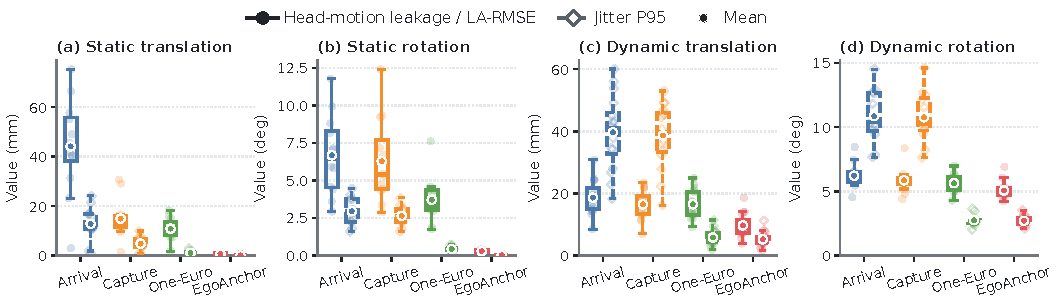
\includegraphics[width=\textwidth]{figures/panels/figure2_exp1_behavior.pdf}
  \caption{Error distributions for the four runtime configurations in Experiment 1. (a,b) P95 head-motion coupling error and stationary jitter for translation and rotation under stationary conditions; (c,d) LA-RMSE and P95 residual jitter during continuous motion. Light points denote individual repeated measurements; boxes and center lines show the cross-repetition IQR and median; dark markers show the mean. Lower is better. EgoAnchor has the lowest plotted static errors and LA-RMSE, with dynamic residual jitter close to One-Euro.}
  \label{fig:exp1-final}
\end{figure*}

\subsubsection{Static Registration}

\begin{table}[t]
\centering
\caption{Static registration metrics in Experiment 1. Each cell reports the cross-repetition median as translation/rotation, with P95 computed within each test sequence. $\downarrow$ indicates lower is better; bold marks the best channel value. Cross-repetition distributions appear in Fig.~\ref{fig:exp1-final}(a,b).}
\label{tab:exp1-static}
\begin{tabular}{@{}lccc@{}}
\toprule
Method & \shortstack{Head-motion coupling\,$\downarrow$\\mm/$^\circ$} & \shortstack{Registration error\,$\downarrow$\\mm/$^\circ$} & \shortstack{Stationary jitter\,$\downarrow$\\mm/$^\circ$} \\
\midrule
Arrival   & 43.67/6.49 & 44.31/9.65 & 11.70/2.98 \\
Capture   & 13.03/5.40 & 17.54/8.26 & 4.30/2.60 \\
One-Euro  & 10.65/3.29 & 14.00/6.96 & 0.85/0.40 \\
EgoAnchor & \textbf{0.82}/\textbf{0.33} & \textbf{6.60}/\textbf{4.39} & \textbf{0.06}/\textbf{0.03} \\
\bottomrule
\end{tabular}
\end{table}

Table~\ref{tab:exp1-static} shows that capture-time composition reduces the head-motion coupling error from 43.67~mm/6.49$^\circ$ for Arrival to 13.03~mm/5.40$^\circ$ for Capture. EgoAnchor reaches 0.82~mm/0.33$^\circ$, approximately 92\%/90\% below One-Euro, and has the lowest registration error at 6.60~mm/4.39$^\circ$. It also reduces stationary jitter from One-Euro's 0.85~mm/0.40$^\circ$ to 0.06~mm/0.03$^\circ$. Fig.~\ref{fig:exp1-final}(a,b) shows the corresponding distributions.

\subsubsection{Dynamic Tracking}

\begin{table}[t]
\centering
\caption{Dynamic tracking metrics in Experiment 1. Each cell reports the cross-repetition median as translation/rotation; residual-jitter P95 is computed within each test sequence. $\downarrow$ indicates lower is better; bold marks the best channel value. Cross-repetition distributions appear in Fig.~\ref{fig:exp1-final}(c,d).}
\label{tab:exp1-dynamic}
\setlength{\tabcolsep}{2pt}
\begin{tabular}{@{}lcccc@{}}
\toprule
Method & \shortstack{Effective lag\,$\downarrow$\\ms} & \shortstack{LA-RMSE\,$\downarrow$\\mm/$^\circ$} & \shortstack{CT-RMSE\,$\downarrow$\\mm/$^\circ$} & \shortstack{Residual jitter\,$\downarrow$\\mm/$^\circ$} \\
\midrule
Arrival   & \textbf{202.5}/\textbf{255.0} & 18.57/6.09 & \textbf{84.74}/25.44 & 41.08/10.40 \\
Capture   & 255.0/257.5 & 17.14/5.84 & 103.63/\textbf{25.35} & 39.69/10.26 \\
One-Euro  & 380.0/385.0 & 15.69/5.55 & 117.61/34.10 & 5.25/2.70 \\
EgoAnchor & 360.0/345.0 & \textbf{9.12}/\textbf{4.81} & 125.83/31.88 & \textbf{4.56}/\textbf{2.64} \\
\bottomrule
\end{tabular}
\end{table}

After optimal lag alignment, EgoAnchor has an LA-RMSE of 9.12~mm/4.81$^\circ$, approximately 42\%/13\% below One-Euro (15.69~mm/5.55$^\circ$). Their residual jitter is similar at 4.56~mm/2.64$^\circ$ and 5.25~mm/2.70$^\circ$, respectively, while the LA-RMSE difference is mainly translational (Table~\ref{tab:exp1-dynamic}).

Current-time error shows the opposite tradeoff. Arrival has the lowest effective lag at 202.5/255.0~ms, versus 380.0/385.0~ms for One-Euro and 360.0/345.0~ms for EgoAnchor. Accordingly, translational CT-RMSE rises from 84.74~mm for Arrival to 125.83~mm for EgoAnchor, although EgoAnchor's rotational CT-RMSE remains below One-Euro (31.88$^\circ$ vs. 34.10$^\circ$). Lower lag-aligned residuals therefore accompany greater phase lag.

\subsubsection{State-Transition Response}

\begin{table}[t]
\centering
\caption{State-transition metrics in Experiment 1. Occlusion recovery error is the cross-repetition median of within-sequence P95 translation/rotation; motion onset latency is the median scalar across channels. $\downarrow$ indicates lower is better; bold marks the best value.}
\label{tab:exp1-transition}
\begin{tabular}{@{}lcc@{}}
\toprule
Method & \shortstack{Occlusion recovery error\,$\downarrow$\\mm/$^\circ$} & \shortstack{Motion onset latency\,$\downarrow$\\ms} \\
\midrule
Arrival   & 18.23/18.39 & \textbf{157.0} \\
Capture   & 16.93/18.38 & 263.8 \\
One-Euro  & 10.41/8.66  & 334.0 \\
EgoAnchor & \textbf{4.85}/\textbf{5.52} & 510.4 \\
\bottomrule
\end{tabular}
\end{table}

EgoAnchor reduces occlusion recovery error to 4.85~mm/5.52$^\circ$, approximately 53\%/36\% below One-Euro, but increases motion onset latency from 334.0 to 510.4~ms (Table~\ref{tab:exp1-transition}). This confirms an accuracy--responsiveness tradeoff.

\subsubsection{Qualitative Replay}

\begin{figure}[t]
  \centering
  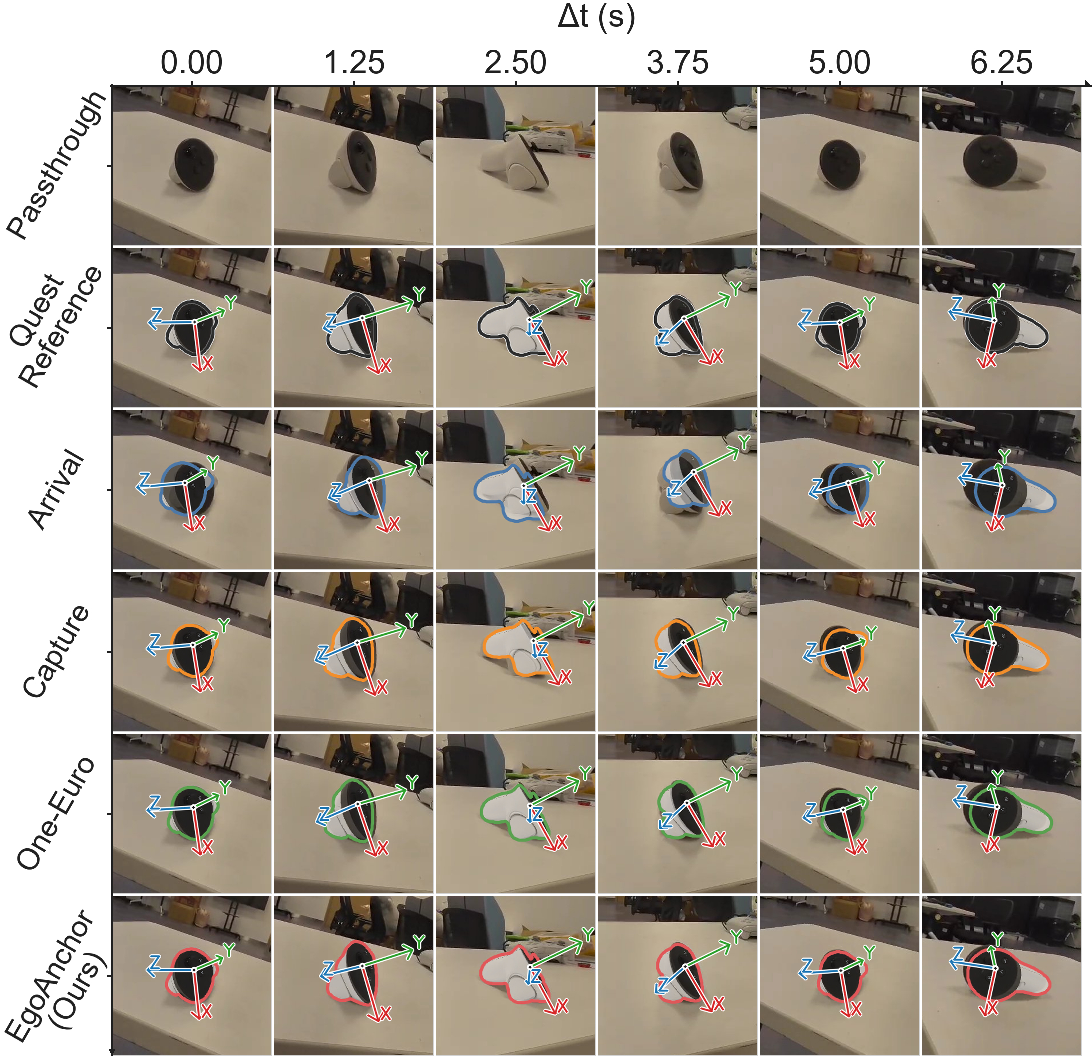
\includegraphics[width=\columnwidth]{figures/replay_grid.pdf}
  \caption{Replay of a continuous sequence in Experiment 1 ($\Delta t=0$--$6.25\,\mathrm{s}$, sampled every $1.25\,\mathrm{s}$). The top two rows show raw passthrough images and the Quest platform tracking reference; the bottom four show anchor projections from Arrival, Capture, One-Euro, and EgoAnchor at the same capture times. Object contours and local axes indicate the estimated 6DoF anchors.}
  \label{fig:exp1-replay}
\end{figure}

Fig.~\ref{fig:exp1-replay} illustrates how the quantitative differences appear during continuous interaction. During head motion, Arrival and Capture show visible spatial offsets. One-Euro reduces some of this displacement, while EgoAnchor maintains lower visual registration error.

\subsection{Experiment 2: Ablation Analysis}

Each ablation uses independently collected paired measurements. We first summarize each repeated trial within its sequence and then report statistics across repetitions. Brackets indicate bootstrap 95\% confidence intervals, and relative changes are reported as paired ratios.

\begin{figure*}[!t]
  \centering
  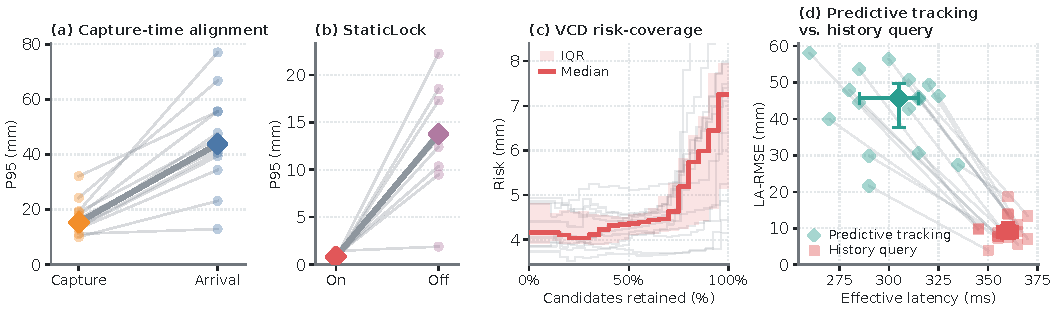
\includegraphics[width=\textwidth]{figures/panels/figure3_exp2_attribution.pdf}
  \caption{Component ablations in Experiment 2. (a) Translational P95 head-motion coupling error using capture-time (Capture) or arrival-time (Arrival) camera poses; (b) the same error with StaticLock enabled (On) or disabled (Off); (c) VCD risk--coverage curves for translational error, with thin gray lines for repetitions and the red line/shading for their median/IQR; (d) translational effective-lag versus LA-RMSE tradeoff for predictive tracking and the historical state query. In (a), (b), and (d), light-gray lines connect paired measurements, and large colored markers/error bars show the cross-repetition median/IQR.}
  \label{fig:exp2-final}
\end{figure*}

Under active head motion, arrival-time rather than capture-time composition increases median P95 head-motion coupling error from 15.38 to 43.75~mm, a paired ratio of 2.69 [2.38, 3.00] (Fig.~\ref{fig:exp2-final}(a)). Disabling StaticLock likewise increases this error for a stationary target from 0.82 to 13.73~mm, a ratio of 17.06 [13.89, 27.52] (Fig.~\ref{fig:exp2-final}(b)).

In Fig.~\ref{fig:exp2-final}(c), selective risk generally rises as coverage expands from high- to low-scoring candidates. Under occlusion, AURC is 4.79 [4.20, 5.13]~mm and full-coverage risk is 7.25 [5.15, 7.95]~mm, indicating that VCD ranks relative geometric reliability.

Predictive tracking reduces effective lag to 305.00/250.00~ms from 360.00/345.00~ms for the historical query, but increases LA-RMSE to 45.64~mm/12.21$^\circ$ from 8.93~mm/4.70$^\circ$ (Fig.~\ref{fig:exp2-final}(d)). Its translational and rotational residuals are 5.46 [4.02, 5.73] and 2.63 [2.44, 2.78] times higher, respectively. Historical queries thus preserve trajectory geometry at the cost of lag.

\subsection{Experiment 3: User Study}

Fig.~\ref{fig:exp3-subjective} shows the paired ratings from 24 participants. Complete statistics for all 12 outcomes, including medians, Wilcoxon statistics, Holm-adjusted $p$ values, and effect sizes, are provided in the supplementary material. The main text focuses on statistically significant or representative results.

\begin{figure*}[!t]
  \centering
  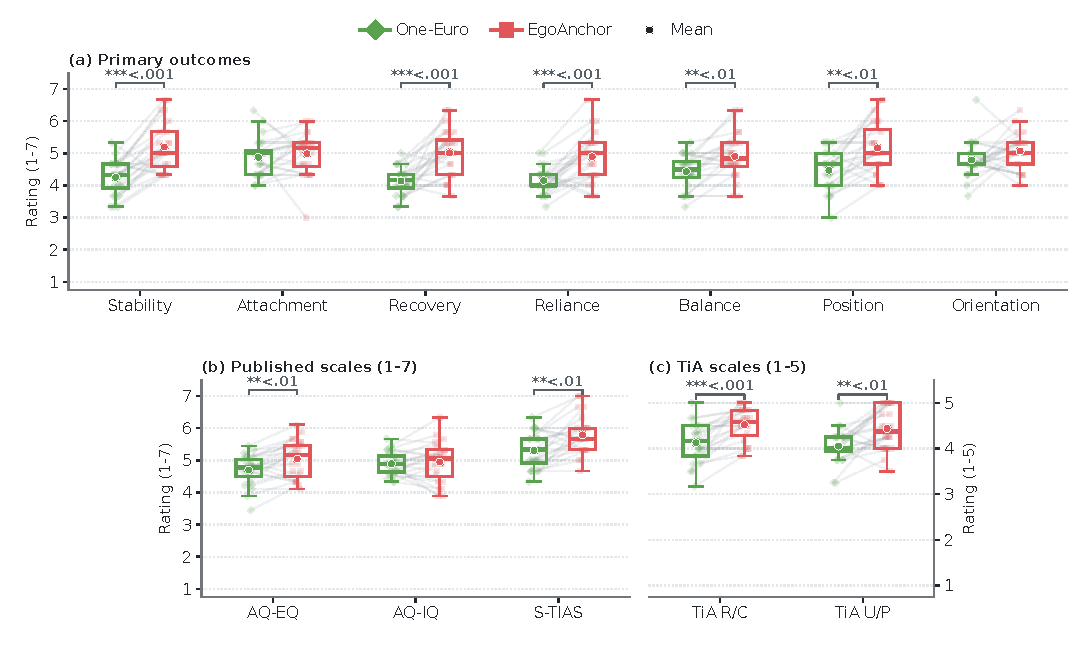
\includegraphics[width=\textwidth]{figures/panels/figure4_exp3_subjective_outcomes.pdf}
  \caption{Within-subject ratings of One-Euro and EgoAnchor from 24 participants. (a) Stationary stability, motion attachment, pose consistency, and recovery consistency; (b) positional correctness, willingness to rely on the system, and the stability--responsiveness tradeoff; (c) AQ Embedding Quality (AQ-EQ), AQ Interaction Quality (AQ-IQ), and overall S-TIAS trust; (d) TiA Reliability/Competence (R/C) and Understanding/Predictability (U/P). Anchor items and AQ scores are averaged within participant across the three objects. Panels (a)--(c) use 7-point scales and (d) a 5-point scale. Light points/gray lines show paired ratings; boxes, center lines, and black points show the IQR, median, and mean. Asterisks denote Holm--Bonferroni-adjusted significance ($^*p_{\mathrm{adj}}<.05$, $^{**}p_{\mathrm{adj}}<.01$, $^{***}p_{\mathrm{adj}}<.001$).}
  \label{fig:exp3-subjective}
\end{figure*}

\subsubsection{Object-Anchoring Experience}

\textbf{Stationary and recovery phases.}
The largest effect sizes among the seven items appear in the stationary and recovery phases. During stationary observation, EgoAnchor has a median rating of 5.00 [4.58, 5.67], higher than the 4.33 [3.92, 4.67] of One-Euro ($W=13.5$, $p_{\mathrm{adj}}<.001$, $r_{\mathrm{rb}}=.90$). After removal of the occluder, the recovery consistency rating is 5.00 [4.33, 5.42] for EgoAnchor and 4.17 [3.92, 4.33] for One-Euro. This difference has the largest effect size among the seven items ($W=6$, $p_{\mathrm{adj}}<.001$, $r_{\mathrm{rb}}=.95$).

\textbf{Continuous motion phase.}
During continuous object manipulation, the perceived difference between the systems narrows. Motion attachment ratings are similar for EgoAnchor at 5.17 [4.58, 5.33] and One-Euro at 5.00 [4.33, 5.08]. Pose consistency ratings are 5.00 [4.67, 5.33] for EgoAnchor and 4.67 [4.67, 5.00] for One-Euro. Neither difference remains statistically significant after Holm correction (attachment: $W=67.5$, $p_{\mathrm{adj}}=.267$, $r_{\mathrm{rb}}=.29$; consistency: $W=81$, $p_{\mathrm{adj}}=.162$, $r_{\mathrm{rb}}=.41$).

\textbf{Overall anchoring judgments.}
All three overall outcomes show statistically significant differences favoring EgoAnchor. Positional correctness is rated 5.00 [4.67, 5.75] for EgoAnchor and 4.67 [4.00, 5.00] for One-Euro ($W=16$, $p_{\mathrm{adj}}=.001$, $r_{\mathrm{rb}}=.85$). Willingness to rely on the system is 5.00 [4.33, 5.33] for EgoAnchor and 4.00 [4.00, 4.33] for One-Euro ($W=16.5$, $p_{\mathrm{adj}}<.001$, $r_{\mathrm{rb}}=.87$). Ratings of the stability--responsiveness tradeoff are 4.83 [4.58, 5.33] and 4.50 [4.25, 4.75], respectively ($W=6$, $p_{\mathrm{adj}}=.003$, $r_{\mathrm{rb}}=.90$).

\subsubsection{Augmentation Quality and Trust}

\textbf{Augmentation quality.}
The AQ results indicate that the main difference lies in perceived visual integration (AQ-EQ) rather than dynamic interaction quality (AQ-IQ). Embedding Quality is 5.17 [4.50, 5.47] for EgoAnchor, higher than the 4.78 [4.50, 5.03] of One-Euro ($W=32$, $p_{\mathrm{adj}}=.004$, $r_{\mathrm{rb}}=.75$). The difference in Interaction Quality does not reach the adjusted significance threshold: EgoAnchor scores 5.06 [4.50, 5.33], and One-Euro scores 4.89 [4.64, 5.14] ($W=102.5$, $p_{\mathrm{adj}}=.446$, $r_{\mathrm{rb}}=.19$).

\textbf{User trust.}
EgoAnchor receives higher ratings on all three trust measures. TiA Reliability/Competence shows the largest effect size ($W=0$, $p_{\mathrm{adj}}<.001$, $r_{\mathrm{rb}}=1.00$), with 4.58 [4.29, 4.83] for EgoAnchor and 4.17 [3.83, 4.50] for One-Euro. For Understanding/Predictability, the corresponding ratings are 4.38 [4.00, 5.00] and 4.00 [3.94, 4.25] ($W=32$, $p_{\mathrm{adj}}=.004$, $r_{\mathrm{rb}}=.75$). Overall S-TIAS trust also shows a significant difference: 5.67 [5.33, 6.00] for EgoAnchor and 5.33 [4.92, 5.67] for One-Euro ($W=22.5$, $p_{\mathrm{adj}}=.004$, $r_{\mathrm{rb}}=.79$).

Reliability analysis shows low internal consistency for AQ Interaction Quality ($\alpha=.504$) and TiA Understanding/Predictability ($\alpha=.565$) under One-Euro. The S-TIAS values are also below .70 for both methods (.672/.697). These scale-level differences should therefore be interpreted with caution. Complete reliability coefficients are provided in the supplementary material.

\textbf{Overall choices.}
In the blinded overall preference question, 62.5\% (15/24) of participants prefer EgoAnchor, four prefer One-Euro, and five report no clear preference. When asked which method they trust directly, 18 select EgoAnchor, one selects One-Euro, and five consider them equivalent. The median preference strength is 4.00 [3.00, 5.00], and confidence in distinguishing the methods is 6.00 [5.00, 7.00]. Three participants reported mild discomfort, and none withdrew from the study.

\section{Discussion}\label{sec:discussion}

\subsection{Technical Implications}

Across the controlled benchmarks and user study, the clearest performance differences arise from explicit recovery of capture-time semantics and dedicated modeling of stationary states, rather than adaptive frame-to-frame smoothing alone. VCD provides an effective reliability ranking for candidate poses, while historical state queries trade response lag for lower geometric trajectory residuals. These objective differences are consistent with the higher EgoAnchor ratings for visual integration, positional correctness, willingness to rely on the system, and interaction trust. A practical egocentric dynamic anchoring system must jointly organize pose geometry, capture timestamps, observation reliability, and asynchronous transmission into an object state that applications can bind to continuously.

EgoAnchor presents a clear engineering tradeoff. It provides higher static stability, more accurate occlusion recovery, and better geometric trajectory fidelity, but has greater motion onset latency. During continuous motion, its instantaneous translational error (CT-RMSE) is higher than that of baselines that output candidates directly. The user study shows a consistent pattern: EgoAnchor's advantages are most apparent during stationary observation and occlusion recovery, as well as in overall trust, whereas subjective differences during continuous manipulation are not statistically significant. Tasks that prioritize spatial alignment, such as physical annotation, assembly guidance, and state monitoring, may favor stability and geometric fidelity. Highly dynamic and latency-sensitive interactions require further optimization of response latency.

\subsection{Limitations and Future Work}

\textbf{Objects and 3D models.}
EgoAnchor currently targets everyday objects with known rigid 3D models. Its anchoring performance depends on target observability and the quality of the model prior. Severe occlusion, weakly textured surfaces, highly reflective or translucent materials, and stereo depth failure can reduce the accuracy of segmentation and pose validation. Nonrigid and deformable objects also fall outside the rigid-object formulation. In addition, because the same 3D model is used for both pose estimation and VCD validation, geometric or scale errors in the model directly introduce systematic error. Future work can investigate lightweight online geometric calibration and automated model-generation pipelines.

\textbf{Evaluation reference and cross-platform comparison.}
Our controlled benchmarks against a hardware-tracked reference use only Meta Quest 3 and do not compare 6DoF tracking across headsets. A primary obstacle is that platforms impose different model origins, axis conventions, scales, and preprocessing requirements, so their pose outputs are defined in different local object frames. Sensor configurations, clock synchronization, and tracking interfaces also differ. Although the Quest 3 controller provides an accurate synchronized reference, its pose still comes from the platform's native visual-inertial tracking rather than absolute ground truth. Future work can establish a unified object-frame calibration and introduce optical motion capture or a high-precision robotic arm for stricter cross-platform evaluation.

\textbf{Deployment and evaluation scope.}
The current system relies on an external high-performance GPU workstation for perception. Network communication and heterogeneous computation introduce inherent latency. Model quantization, distillation, and mobile NPU acceleration may enable lightweight on-device deployment, reducing end-to-end latency and improving performance under fast object manipulation. The controlled benchmark uses the official controller to obtain an accurate tracking reference, while the user study uses three rigid objects to balance object diversity against study duration. Future studies can reuse the static registration, dynamic tracking, and state-transition metrics across more object categories and heterogeneous headsets, contributing to standardized evaluation of dynamic object anchoring~\cite{cheng2024tracking,hu2024applemeta,hu2025xrrealitycheck}.

\section{Conclusion}\label{sec:conclusion}

We present EgoAnchor, an egocentric system for zero-shot dynamic object anchoring in passthrough mixed reality. It transforms asynchronous camera-frame observations into world-frame states at image capture time and maintains reliable object states for the rendering pipeline. In this way, EgoAnchor converts discrete, low-rate visual estimates into continuous and stable spatial anchors that support occlusion recovery. Controlled benchmarks and ablations show lower static registration error, occlusion recovery error, and geometric trajectory residuals than the baselines, but higher motion onset latency. The within-subject study with 24 participants further shows higher ratings for perceived visual integration, interaction trust, and willingness to rely on EgoAnchor.

Converting visually estimated poses into usable object-level spatial anchors requires more than accurate single-frame pose estimation. It also requires systematic runtime modeling of temporal semantics, perceptual uncertainty, and the state lifecycle. As open-vocabulary foundation models, rapid 3D generation, and mobile computing continue to advance, a perception-runtime architecture can extend high-fidelity dynamic anchoring to more everyday objects and natural interaction scenarios.

\acknowledgments{
  OpenAI ChatGPT was used to assist with English translation and language editing. The authors reviewed and verified all changes.
}
% Camera-ready only: This work was supported by the National Natural Science
% Foundation of China under Grant 62377004.

\bibliographystyle{abbrv-doi-hyperref-narrow}
\bibliography{egoanchor_cn_refs}

\end{document}
